\documentclass{beamer}

\mode<presentation>
{
  \usetheme{Warsaw}
  \setbeamercovered{invisible}
}

\setbeamertemplate{navigation symbols}{}

\graphicspath{{./images/}}

\usepackage[english]{babel}
\usepackage{times}
\usepackage[latin1]{inputenc}
\usepackage[T1]{fontenc}
\usepackage{lmodern}
\usepackage{amsmath,amsthm,amssymb}
\usepackage{hyperref}
\usepackage{nccfoots}
\usepackage{subfigure}
\usepackage{outlines}

\newcommand{\MCMC}{$\mathrm{MCMC}$ }
\newcommand{\nni}{\mathrm{NNI}}

\setbeamercolor{author}{fg=brown}
\setbeamercolor{date}{fg=white}
\setbeamercolor{institute}{fg=white}

\title[\url{https://gavruskin.github.io/talks/2016_GSA.pdf}]{The space of sampled ancestor trees\\
@GSA2016}
\author[Alex Gavryushkin \hspace{80pt} These slides:]{\large{Alex Gavryushkin}}
\institute{
\includegraphics[height=7.5mm]{ETH_logo_white}\\
\vskip10pt
\large{Joint work with\\
Alexei Drummond, the University of Auckland, NZ,\\
Erick Matsen and Chris Whidden,\\
Fred Hutch Cancer Research Center, Seattle, WA, USA}}
\date{September 28, 2016}


\begin{document}

{
\usebackgroundtemplate{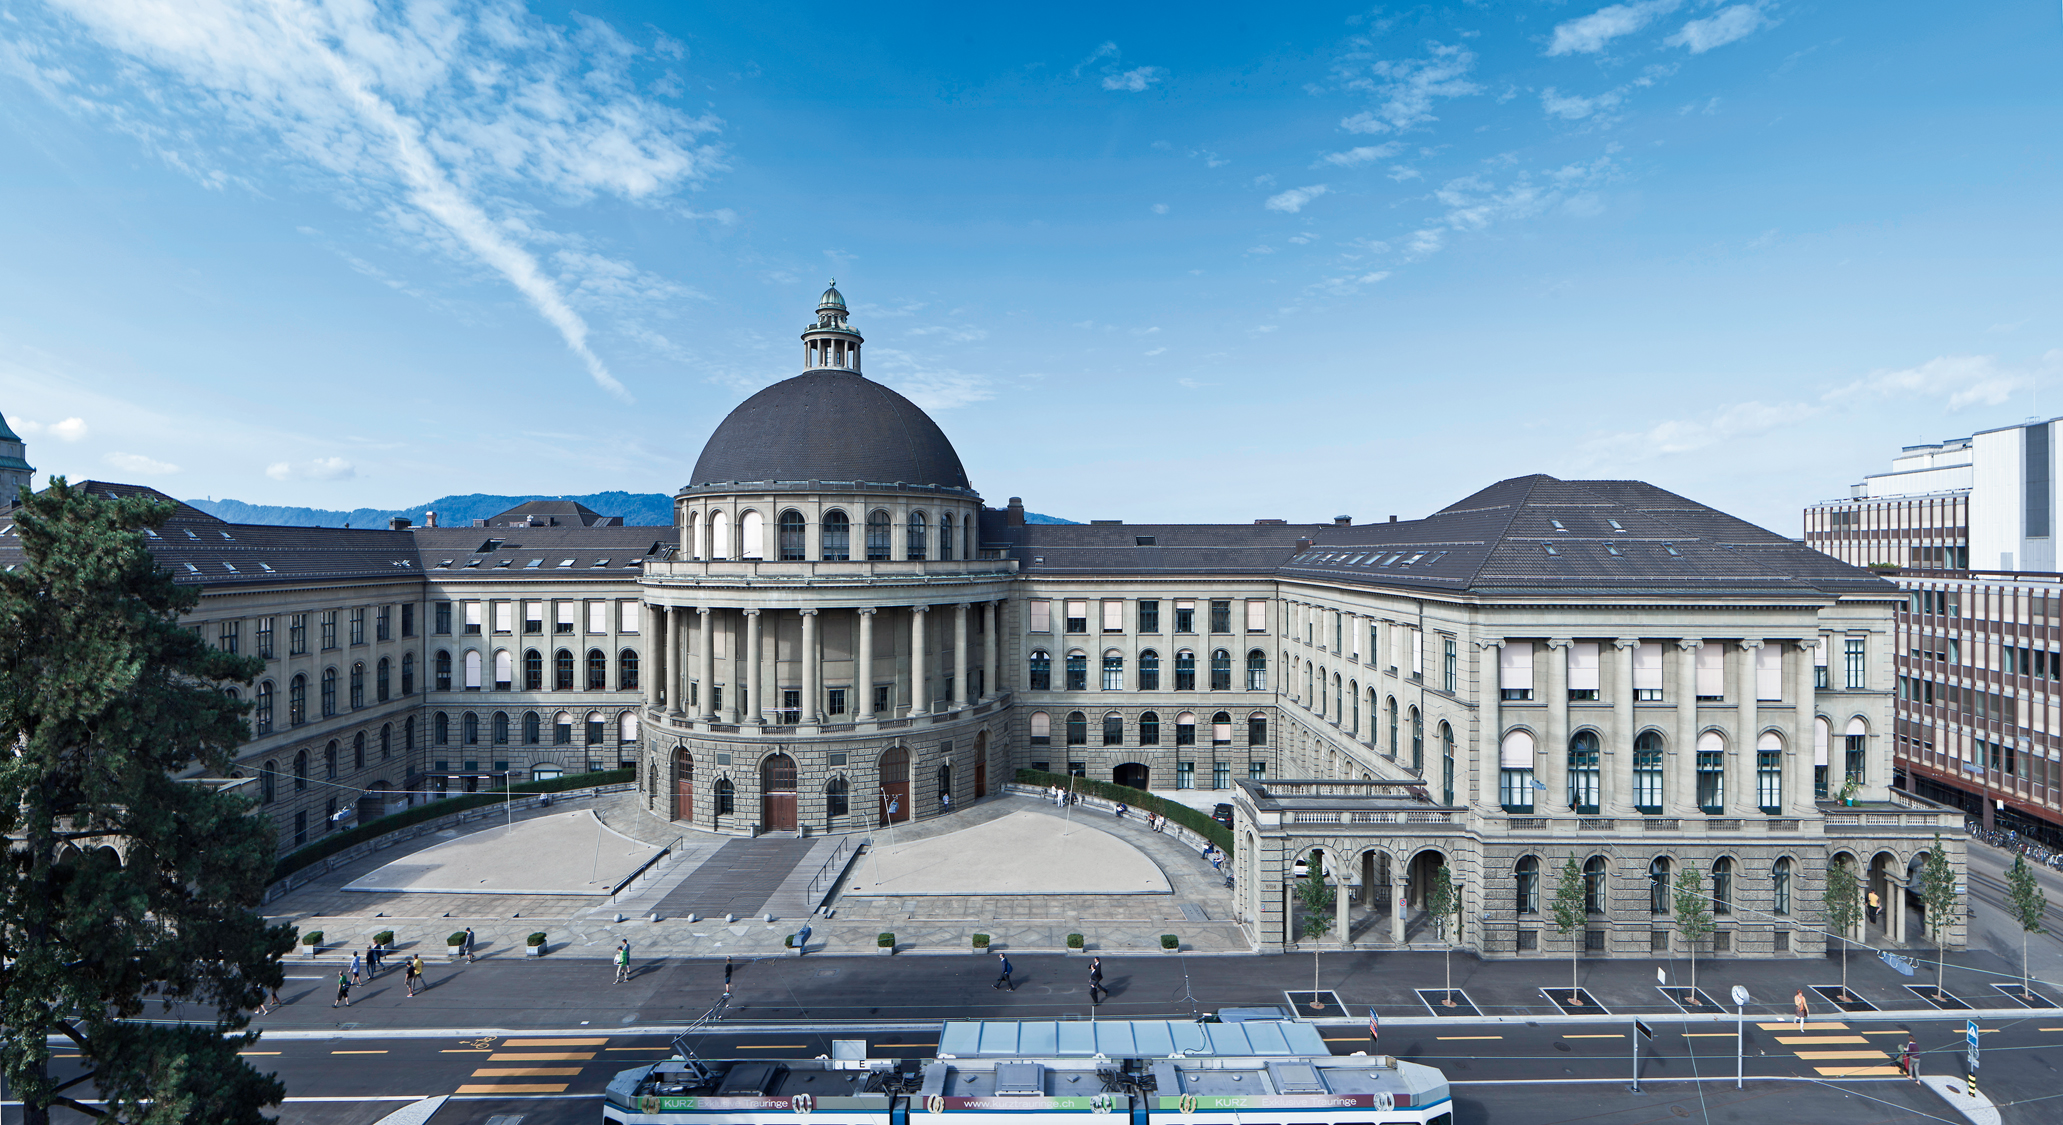
\includegraphics[height=\paperheight]{ETH_image_covered}}
\begin{frame}[plain]
\setbeamertemplate{footline}{}
\titlepage
\end{frame}
}

\addtocounter{framenumber}{-1}
\addtobeamertemplate{navigation symbols}{}{
	\usebeamerfont{footline}
	\usebeamercolor[fg]{footline}
	\hspace{1em}
	\insertframenumber/\inserttotalframenumber
}

\begin{frame}{Motivation}
\begin{block}

\begin{outline}
\1 General statistics is at least $5$ years ahead of phylostatistics.
\pause
\1 The discrete component of tree space is \emph{the} bottleneck for tree search algorithms.
\pause
\1 What's wrong with trees?
\end{outline}
\end{block}

\pause

\begin{block}{Same as above but with a mortarboard on}
\begin{outline}
\1 \MCMC algorithms
	\2 Improving efficiency $=$ smart proposals
	\2 Point estimates AKA posterior summary
\1 Tree search methods in general
	\2 Semi-convergence
	\2 Valleys
	\2 Terraces
\end{outline}
\end{block}
\end{frame}

\begin{frame}
\begin{block}{Sampled ancestor tree}
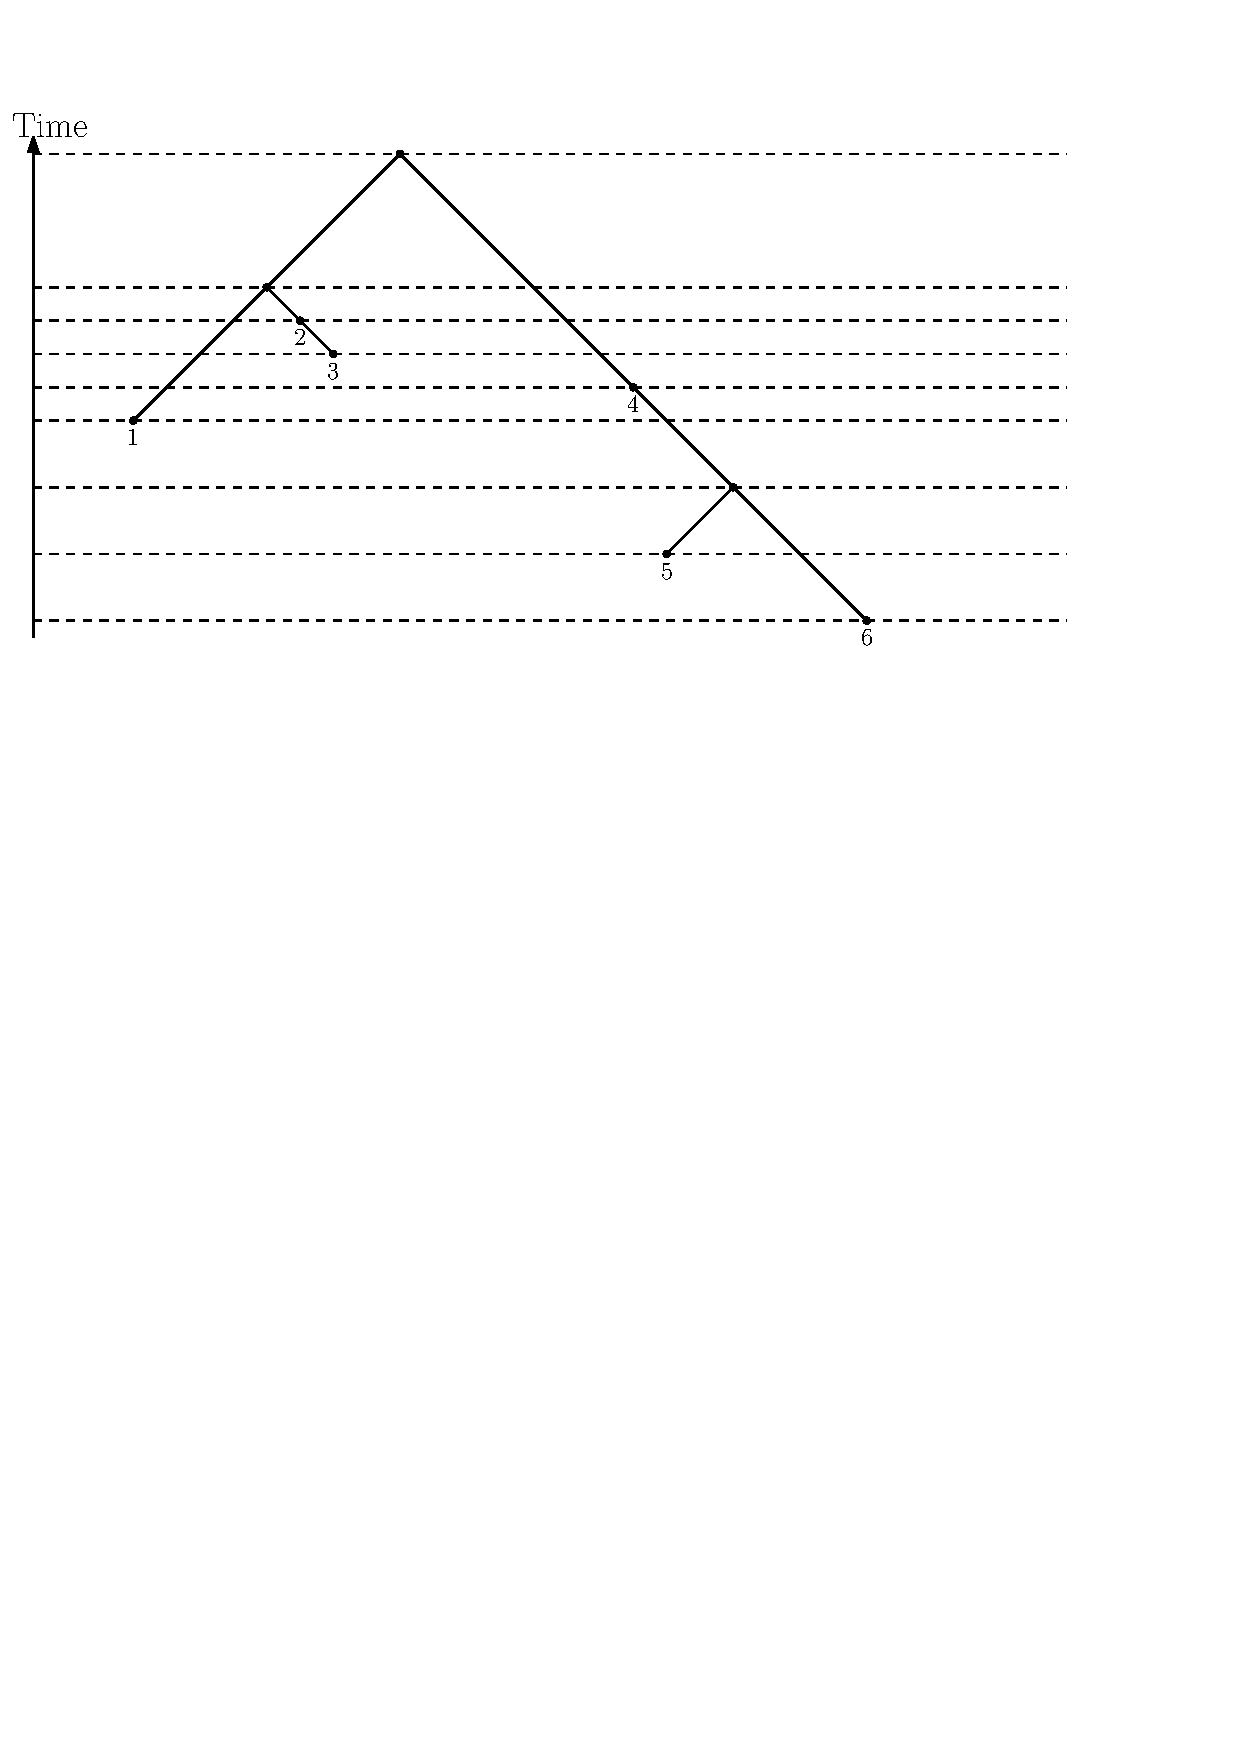
\includegraphics[width=\framewidth]{SampledAncestorTree}
\end{block}
\end{frame}

\begin{frame}
\begin{block}{Sampled ancestor tree graph}
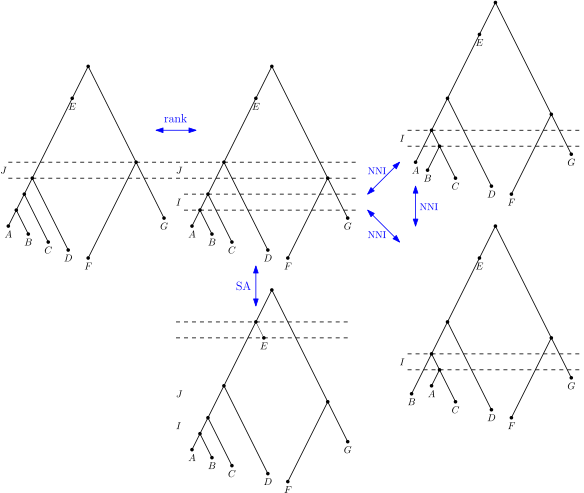
\includegraphics[width=0.8\framewidth]{SAT}
\end{block}
\end{frame}

\begin{frame}{Graph $=$ Metric space}
\pause
\centering

\includegraphics[width=0.4\framewidth]{facepalm1}
\end{frame}

\begin{frame}{What's wrong with the tree space?}
\begin{block}{Answer}
\begin{outline}
\1 Over $25$ years to solve the complexity problem!
\pause
\1 Over 7 erroneous ``solutions'' published on the way!
\end{outline}
\end{block}

\vskip20pt
\pause

\begin{block}{}
I'm talking about the $\nni$ graph here.
\end{block}
\end{frame}

\begin{frame}{What is actually ``wrong''}
\begin{block}{The Split Theorem}
\centering
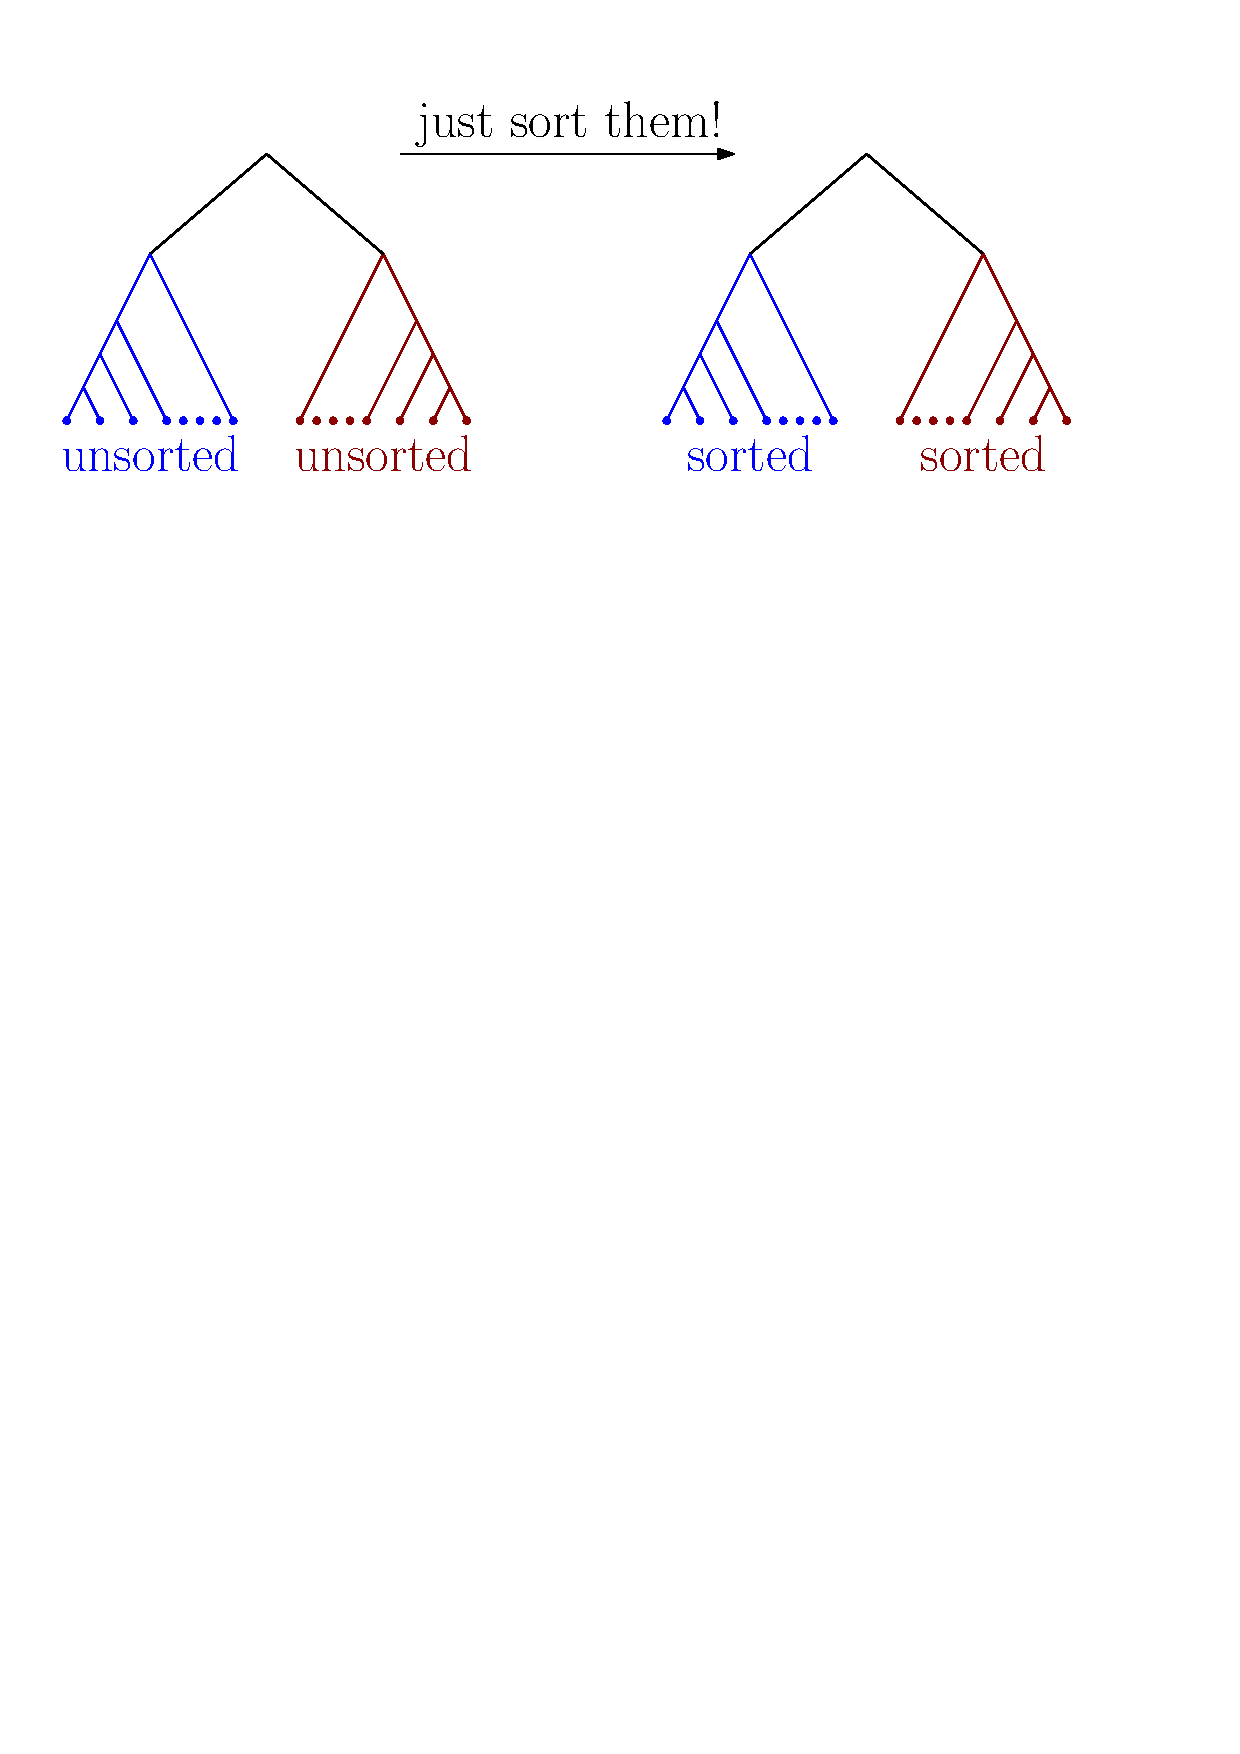
\includegraphics[width=0.9\framewidth]{merge_and_sort_trick}
\end{block}
\end{frame}

\begin{frame}{What is actually ``wrong''}
\begin{block}{Merge and sort trick}
\centering
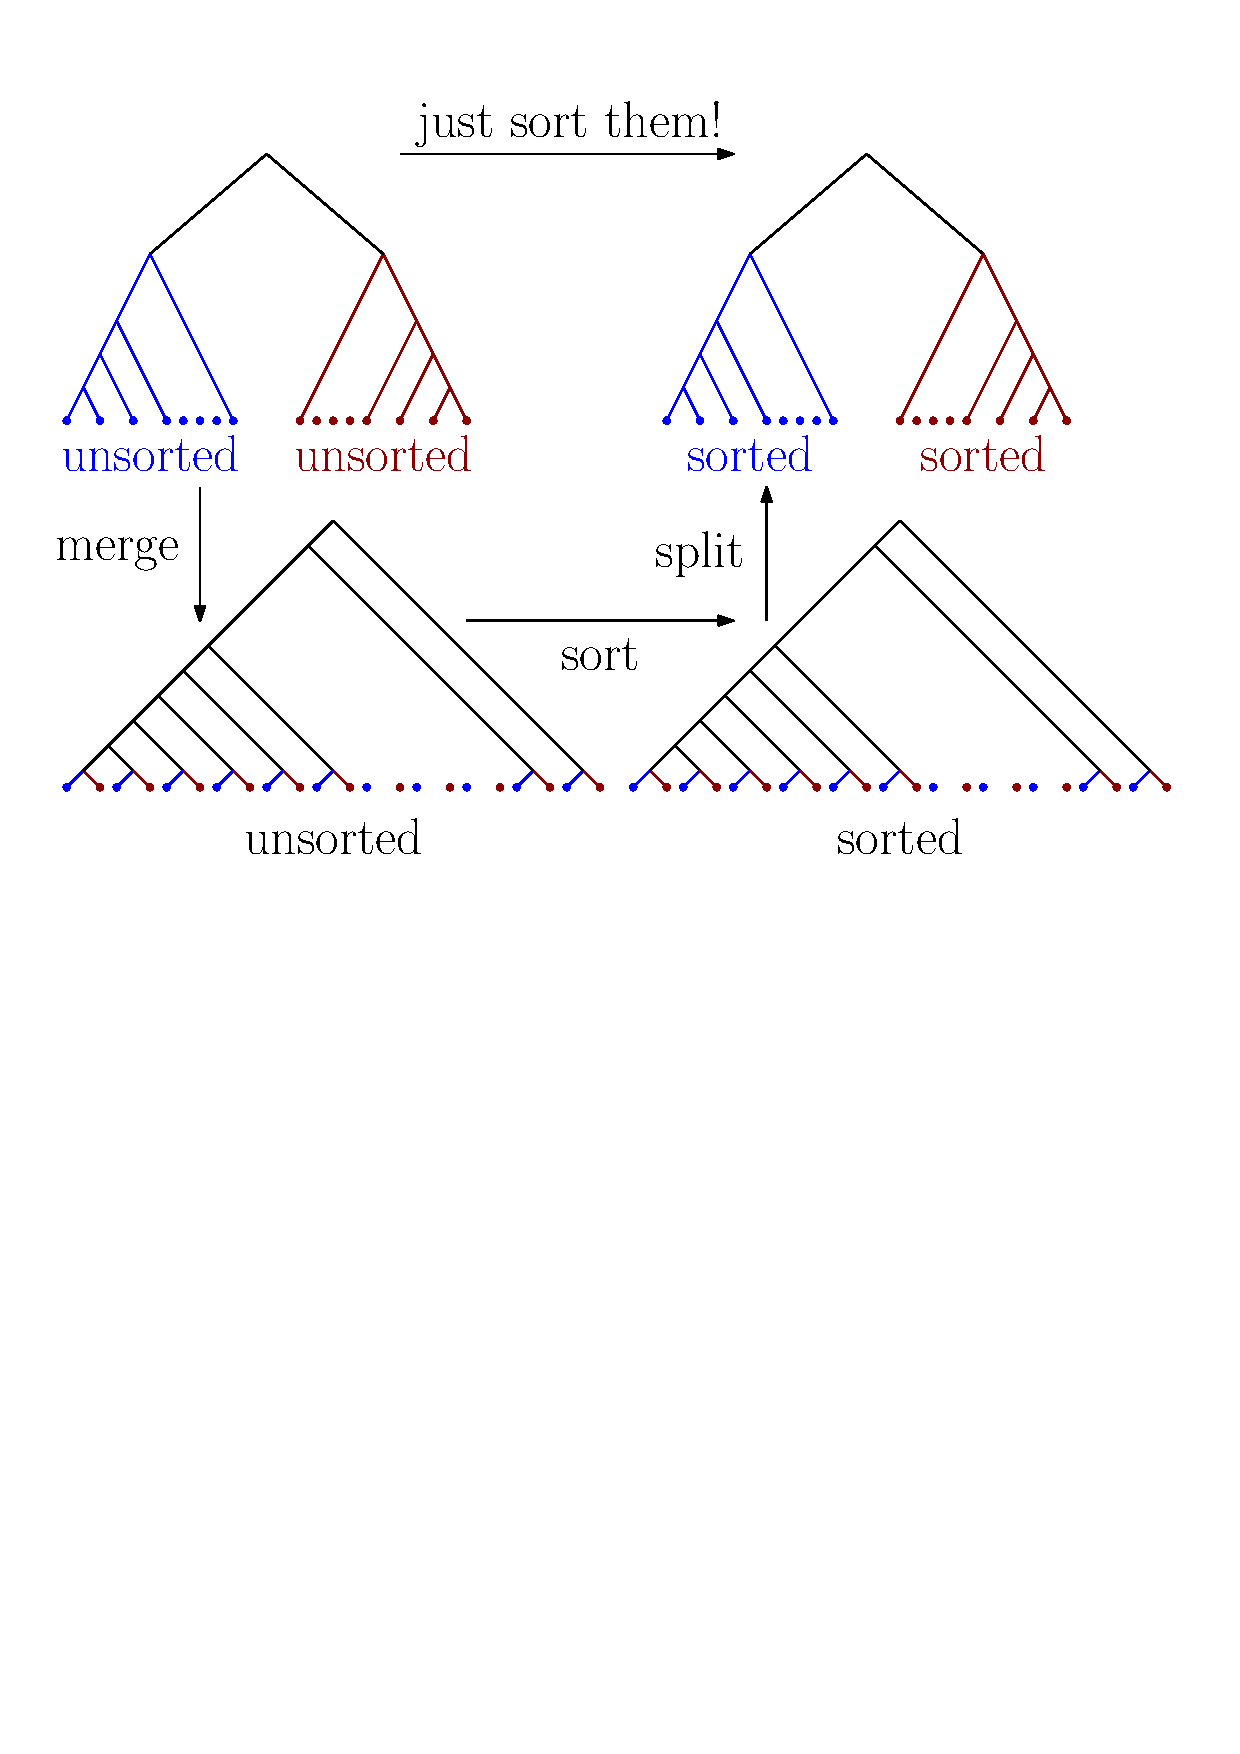
\includegraphics[width=0.9\framewidth]{merge_and_sort_trick_solution}
\end{block}
\end{frame}

\begin{frame}{Good news!}
\begin{block}{Sampled ancestor trees (the $\mathrm{SANNI}$ graph) free from all these\\
(G, Whidden, Matsen. {\em bioRxiv,} 2016)}
\begin{outline}
\1 Split Theorem. Tick.
\1 Merge and sort trick. Tick.
\end{outline}
\end{block}

\pause

\begin{block}{Even more good news}
Efficient approximate algorithm for computing shortest $\mathrm{SANNI}$-paths.
\end{block}
\end{frame}

\begin{frame}{What about branch lengths?}
\begin{block}{G and Drummond. \emph{JTB,} 2016}
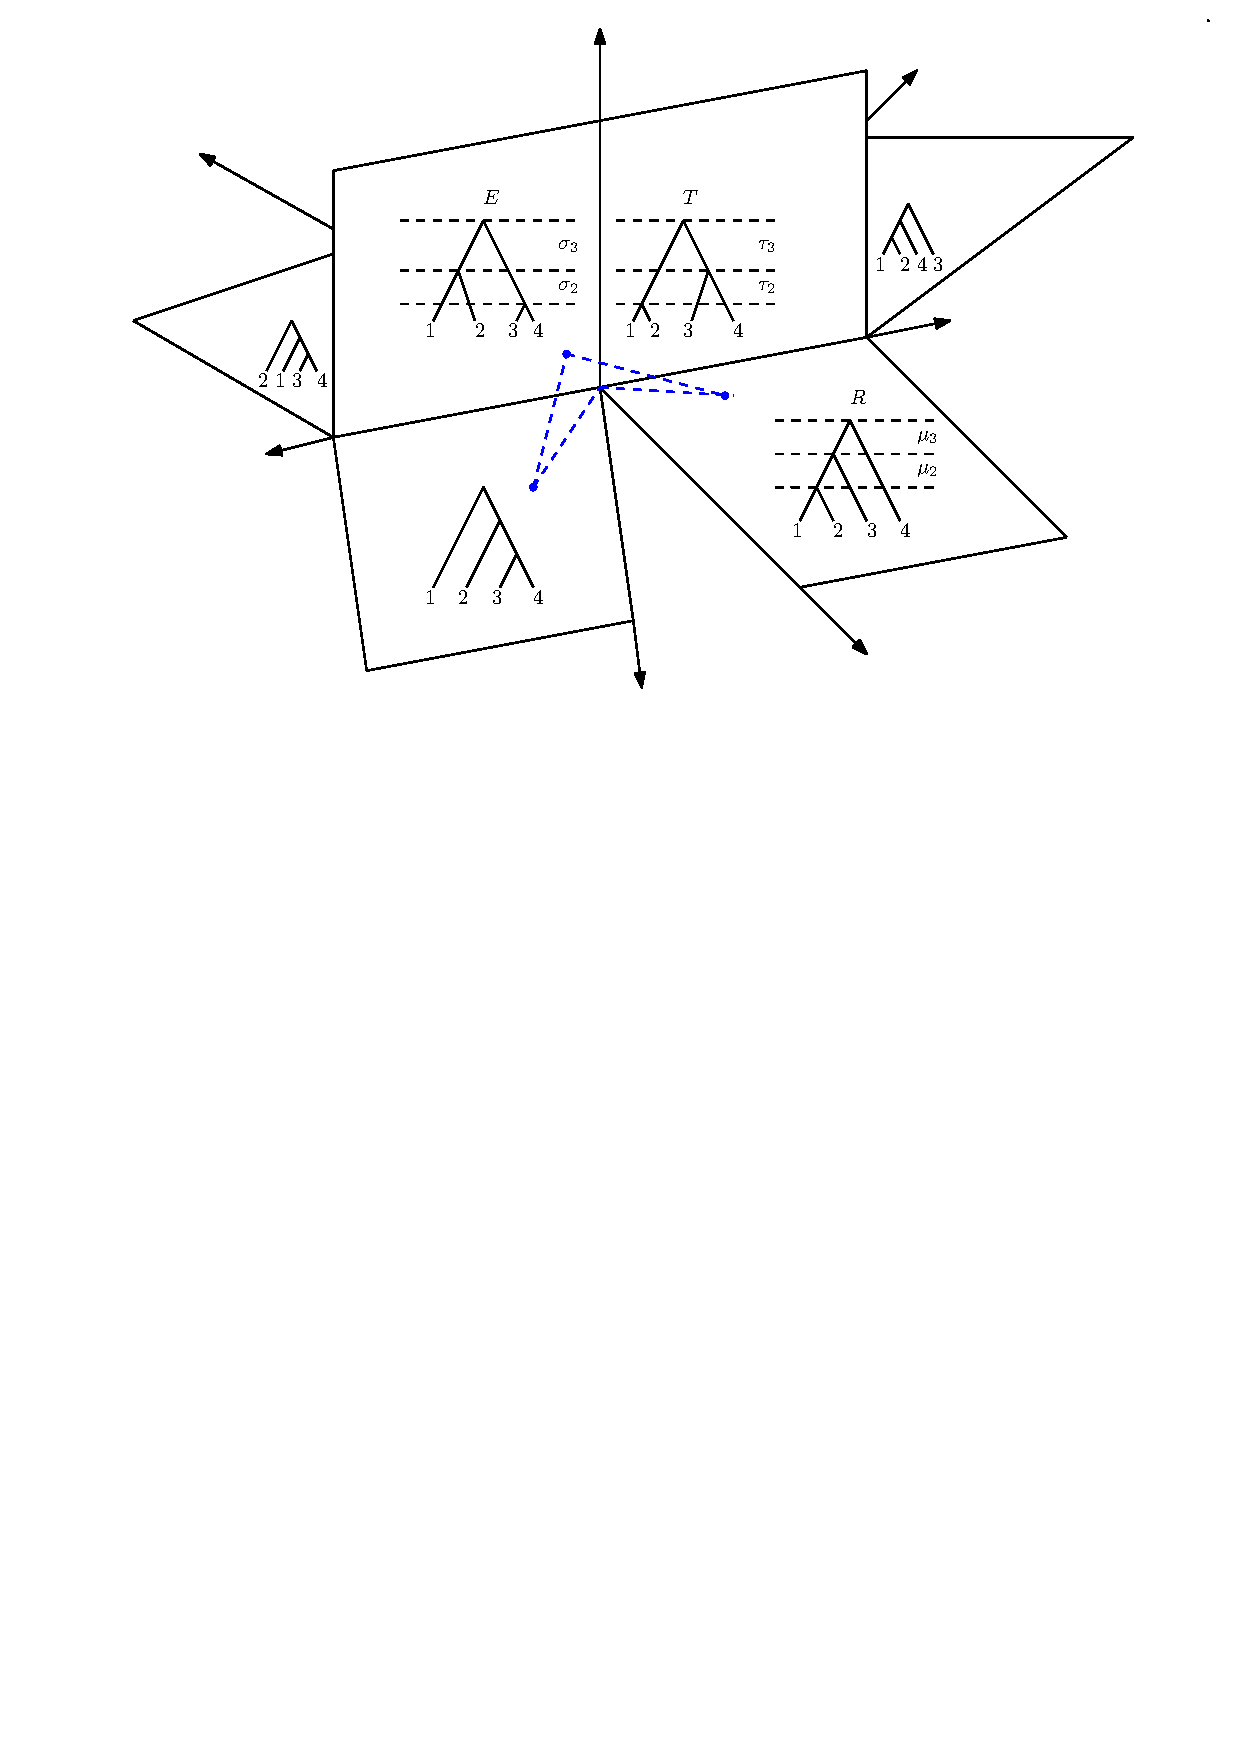
\includegraphics[width=\framewidth]{tauSpace}
\end{block}
\end{frame}

\begin{frame}{Looks like a problem}
\begin{block}{Trees have different dimensions}
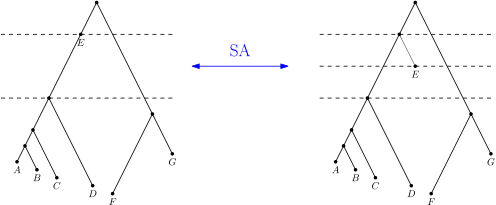
\includegraphics[width=\framewidth]{SAT_dimension}
\end{block}
\end{frame}

\begin{frame}{Branch lengths are fine too!}
\begin{block}{Stadler (\emph{JTB,} 2010) is cheating${}^*$ anyway...}
...\ so we can too: introduce ``imaginary'' nodes:\\
\vskip10pt
\centering
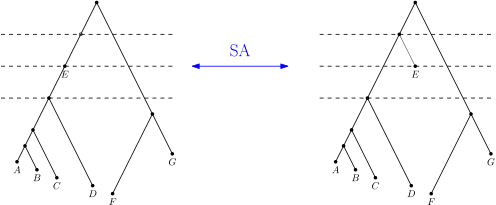
\includegraphics[width=\framewidth]{SAT_dimension_solved}
\end{block}

\pause

\begin{block}{}
${}^*$by putting non-zero probability mass onto facets of the space
\end{block}
\end{frame}

\begin{frame}{What we've done}

\begin{block}{}
\begin{outline}
\1 Introduced the $\mathrm{SANNI}$ graph on ranked sampled ancestor trees (to the best of our knowledge)
\1 Sampled ancestor trees and classical phylogenetic trees have different geometric and algorithmic properties
\1 Often, geometric and algorithmic results for classical trees do not scale to sampled ancestor trees
\1 Natural and efficient data structures
\1 Connections to other areas of math
\pause
\1 Failed to prove that $\mathrm{SANNI}$ is $\mathrm{NP}$-hard
\end{outline}
\end{block}
\end{frame}

\begin{frame}{References}
\thebibliography{9}
\bibliographystyle{alpha}

\scriptsize

\bibitem{LTZ}
Li, Tromp, and Zhang
\newblock Some Notes on the Nearest Neighbour Interchange Distance.
\newblock \emph{Computing and Combinatorics,} 343--351, 1996.

\bibitem{dasgupta}
Dasgupta, He, Jiang, Li, Tromp, and Zhang
\newblock On Computing the Nearest Neighbor Interchange Distance
\newblock \emph{Discrete Mathematical Problems with Medical Applications,} Vol.\,55, 2000.

\bibitem{Gavruskin2015}
Alex Gavryushkin and Alexei Drummond
\newblock The space of ultrametric phylogenetic trees
\newblock \emph{Journal of Theoretical Biology,} Vol.\,402, 197--208, 2016

\bibitem{chrisErickG2015}
Alex Gavryushkin, Chris Whidden, and Frederick A.\ Matsen IV
\newblock Combinatorics of discrete time-trees: algorithmic insights and open problems
\newblock {\em bioRxiv,} 2016 ~~~ $\leftarrow$ ~~~ available as a blog post by Matsen

\bibitem{GavryushkinGitHub}
\url{https://github.com/gavruskin/tauGeodesic}

\bibitem{GavryushkinGitHub2}
\url{https://github.com/gavruskin/tTauCurvature}
\end{frame}

\begin{frame}{\href{http://alex.gavruskin.com/pictures/}{\Large{Thank you for your attention!}}}
\begin{block}{Funding}
\centering

\includegraphics[width=\framewidth]{UniAuckland.png}
\end{block}
\end{frame}

\end{document}

